% Schematic composition of maps in the two-endpoint return.
% Arrows are map order, not phase-plane trajectories.
\begin{figure}[H]
\centering
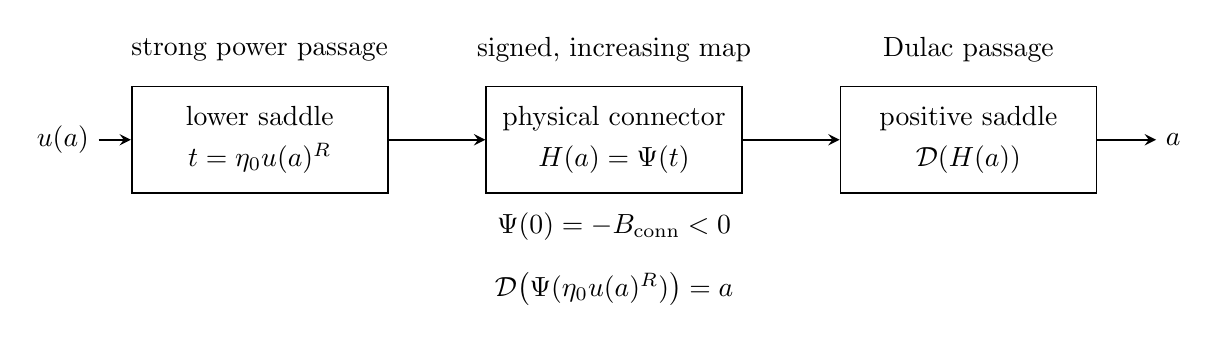
\begin{tikzpicture}[x=10mm,y=10mm,>=stealth,
  every node/.style={font=\fontsize{10}{12}\selectfont},
  block/.style={draw,line width=.6pt,minimum width=3.25cm,
    minimum height=1.35cm,align=center},
  map/.style={->,line width=.8pt}]
  \node (source) at (0,.2) {$u(a)$};
  \node[block] (lower) at (2.5,.2)
    {lower saddle\\[1mm]$t=\eta_0u(a)^R$};
  \node[block] (connector) at (7.0,.2)
    {physical connector\\[1mm]$H(a)=\Psi(t)$};
  \node[block] (positive) at (11.5,.2)
    {positive saddle\\[1mm]$\mathcal D(H(a))$};
  \node (target) at (14.1,.2) {$a$};
  \draw[map] (source)--(lower);
  \draw[map] (lower)--(connector);
  \draw[map] (connector)--(positive);
  \draw[map] (positive)--(target);
  \node at (2.5,1.35) {strong power passage};
  \node at (7.0,1.35) {signed, increasing map};
  \node at (11.5,1.35) {Dulac passage};
  \node at (7.0,-.9) {$\Psi(0)=-B_{\rm conn}<0$};
  \node at (7,-1.7)
    {$\mathcal D\!\left(\Psi(\eta_0u(a)^R)\right)=a$};
\end{tikzpicture}
\caption{Schematic composition of the complete negative-forcing two-endpoint return.
The arrows show the order of scalar maps, not phase-plane trajectories.
The full signed connector $\Psi$, with $\Psi(0)=-B_{\rm conn}<0$, is retained
in $H(a)=\Psi(\eta_0u(a)^R)$. The positive-saddle Dulac map is used on the
returning domain $H(a)>0$.}
\label{fig:two-saddle-connector}
\end{figure}
